\documentclass[review]{elsarticle}

\usepackage[utf8]{inputenc}

\usepackage{lineno,hyperref}
\modulolinenumbers[5]

\usepackage{gensymb}

%% Necessary for multiple images in a row
\usepackage{graphicx}
\usepackage{placeins}
\usepackage{caption}
\usepackage{subcaption}
\usepackage{booktabs} % for table* env.
\usepackage{multirow} % for row spanning

%% Para los colores de las anotaciones, eliminar para vf!!
\usepackage{color}
\usepackage{soul} % para tachar palabras
\setstcolor{teal}

\usepackage{float}
\usepackage{wasysym} % For the circles in the table
\usepackage{threeparttable}
\newcommand\tab[1][0.5cm]{\hspace*{#1}}

%% Commands for table format
%\newcolumntype{R}[2]{%
%    >{\adjustbox{angle=#1,lap=\width-(#2)}\bgroup}%
%    l%
%    <{\egroup}%
%}
\newcommand*\rot{\multicolumn{1}{R{90}{1em}}}%
\newcommand{\ra}[1]{\renewcommand{\arraystretch}{#1}}

%% --------------------------- Old revision system -------------------------------
%% Change to final when definitive version of the paper will be generated.
%%\usepackage[draft, lang=spanish, mode=multiuser]{fixme}

%%\FXRegisterAuthor{kcmd}{kenv}{klyone}
%%\FXRegisterAuthor{jcmd}{jenv}{jda}
%%\FXRegisterAuthor{fcmd}{fenv}{felipetg}
%% --------------------------- Old revision system -------------------------------

%% Commands for the annotations
\usepackage[spanish, colorinlistoftodos, textsize=tiny]{todonotes}

%% Standard notes
\newcommand{\ftglnote}[1]{\todo[bordercolor=violet, backgroundcolor=yellow]{#1}}
\newcommand{\klyonelnote}[1]{\todo[bordercolor=red, backgroundcolor=yellow]{#1}}
\newcommand{\ftgnote}[1]{\todo[bordercolor=violet, backgroundcolor=yellow, noline]{#1}}
\newcommand{\klyonenote}[1]{\todo[bordercolor=red, backgroundcolor=yellow, noline]{#1}}
\newcommand{\gutinote}[1]{\todo[bordercolor=green, backgroundcolor=yellow, noline]{#1}}

%% Notes with high level of importance
\newcommand{\ftglwarning}[1]{\todo[bordercolor=violet, backgroundcolor=orange]{#1}}
\newcommand{\klyonelwarning}[1]{\todo[bordercolor=red, backgroundcolor=orange]{#1}}
\newcommand{\ftgwarning}[1]{\todo[bordercolor=violet, backgroundcolor=orange, noline]{#1}}
\newcommand{\klyonewarning}[1]{\todo[bordercolor=red, backgroundcolor=orange, noline]{#1}}

\journal{Journal of Network and Computer Applications}

%%%%%%%%%%%%%%%%%%%%%%%
%% Elsevier bibliography styles
%%%%%%%%%%%%%%%%%%%%%%%
%% To change the style, put a % in front of the second line of the current style and
%% remove the % from the second line of the style you would like to use.
%%%%%%%%%%%%%%%%%%%%%%%

%% Numbered
%\bibliographystyle{model1-num-names}

%% Numbered without titles
%\bibliographystyle{model1a-num-names}

%% Harvard
%\bibliographystyle{model2-names.bst}\biboptions{authoryear}

%% Vancouver numbered
%\usepackage{numcompress}\bibliographystyle{model3-num-names}

%% Vancouver name/year
%\usepackage{numcompress}\bibliographystyle{model4-names}\biboptions{authoryear}

%% APA style
%\bibliographystyle{model5-names}\biboptions{authoryear}

%% AMA style
%\usepackage{numcompress}\bibliographystyle{model6-num-names}

%% `Elsevier LaTeX' style
\bibliographystyle{elsarticle-num}
%%%%%%%%%%%%%%%%%%%%%%%

\begin{document}

\begin{frontmatter}

\title{A fully programmable White-Rabbit node for the SKA Telescope PPS distribution system}
%\title{Elsevier \LaTeX\ template\tnoteref{mytitlenote}}
%\tnotetext[mytitlenote]{Fully documented templates are available in the elsarticle package on %\href{http://www.ctan.org/tex-archive/macros/latex/contrib/elsarticle}{CTAN}.}

%% Group authors per affiliation:
%\author{Elsevier\fnref{myfootnote}}
%\address{Radarweg 29, Amsterdam}
%\fntext[myfootnote]{Since 1880.}

%% Group authors per affiliation:
\author{Miguel Jiménez-López}
\ead{klyone@ugr.es}
\author{Felipe Torres-González}
\ead{felipetg@ugr.es}
\author{Jose Luis Gutiérrez-Rivas}
\ead{jlgutierrez@ugr.es}
\author{Manolo Rodríguez-Álvarez}
\ead{manolo@ugr.es}
\author{Javier Díaz}
\ead{jda@ugr.es}
\address{CITIC, ETSIIT, University of Granada, Spain}

%% or include affiliations in footnotes:
%\author[mymainaddress,mysecondaryaddress]{Elsevier Inc}
%\ead[url]{www.elsevier.com}

%\author[mysecondaryaddress]{Global Customer 
%Service\corref{mycorrespondingauthor}}
\cortext[mycorrespondingauthor]{Corresponding author.}

%\address[mymainaddress]{1600 John F Kennedy Boulevard, Philadelphia}
%\address[mysecondaryaddress]{360 Park Avenue South, New York}

%\listoffixmes

\begin{abstract} 
	Distributed data acquisition systems (DAQ) are in charge of converting different analogue environment signals into digital values to perform control and monitor tasks. They require a computer network technology to share data between their different elements. One of the main issues related to the DAQ systems is to match data with the specific events under study. A possible solution is to include an event synchronisation technology such as Network Time Protocol (NTP), Precise Time Protocol (PTP) or White Rabbit (WR).
	This contribution proposes a high performance distributed timing system based on WR technology. We focus on the Square Kilometre Array (SKA) project as example of distributed DAQ system. The SKA will be the largest radio-telescope of the world and it will be located in two different geographical areas (South-Africa and Australia/New Zealand). SKA Telescope will be composed of hundred of antennas and their individual observations will be combined acting as a single big antenna. To achieve this aim, they must be synchronised to the same reference very accurately, being required a synchronisation performance below 2 ns. This accuracy is not achievable by current standard synchronisation technologies such as NTP or PTP. Under this context, the authors propose the WR Zynq Embedded Node (WR-ZEN) platform as a candidate for the SKA's Pulse Per Second (PPS) distribution system.  It is a new design based on a Field Programmable Gate Array System-on-Chip (FPGA-SoC) that integrates the WR technology, thus enabling sub-nanosecond accuracy. It presents several advantages compared to older WR implementations such as an enhanced clocking circuitry and high-level software capabilities. Finally, the WR-ZEN has been evaluated in different scenarios to demonstrate its timing performance in dynamic environment conditions fulfilling the SKA Telescope timing requirements for PPS distribution. 
\end{abstract}

\begin{keyword}
	Square Kilometre Array, White Rabbit, Synchronization, Network, Gigabit 
	Ethernet, Optical fiber
\end{keyword}

\end{frontmatter}

\linenumbers

\section{Introduction} \label{sec:intro}

Nowadays, there are many industrial \cite{daq:res} and scientific applications \cite{daq:sensor-networks} that require DAQ systems \cite{daq:book1}. Their main purpose is the study of physical phenomenons converting the analogue environment signals into digital values. They solve the problem of analogue signal distribution by utilizing  widely-used digital network technologies such as Ethernet. Furthermore, the communication link can include not only the digitalized sensors data but also control and auxiliary information.
Distributed DAQ systems include a specific node that is responsible for receiving, processing and extracting critical information related to a certain event. Due to the distributed nature of DAQ systems, it becomes mandatory to define some mechanisms to match events data acquired in different nodes. One possible solution is to implement a synchronisation mechanism in the distributed DAQ network sharing the time information between different nodes. Time synchronisation makes possible the identification of events by the time they occurred.

There are many mechanisms to distribute time information and signals in distributed systems. Some of them use Global Navigation Satellite System (GNSS) receivers to get timing from Satellites (Global Positioning System (GPS), Global'naya Navigatsionnaya Sputnikovaya Sistema (GLONASS)  \cite{glonass:website}, Galileo \cite{gsa:galileo}) meanwhile others use wired protocols (National Marine Electronics Association (NMEA) Protocol, Inter-range instrumentation group time code (IRIG-B)) to disseminate the time reference through the network. The GPS approach is widely used in systems that require accurate synchronisation since devices can be easily connected to different GPS receivers. The main concern related to GPS systems regards to their exposure to jamming and spoofing attacks. However, some studies reveal that wire synchronisation mechanisms can help to reduce the negative effects related to the interference \cite{NOURA2016130}. Alternatively and thanks to the popularity of Ethernet packet networks, timing protocols are being imposed gradually as the main time transfer solution. Low performance protocols such as NTP \cite{ntf:ntp_std}, are widely used in standard applications while the industrial domain requires a more precise protocol like the IEEE-1588v2 (known as PTPv2) \cite{ieee:ieee1588_std} \cite{itu:TG8275_1_Y_1369_1}. PTPv2 is an industrial evolution of NTP, characterised by the utilisation of hardware time-stamping mechanisms that significantly improves time synchronisation accuracy. Typically, NTP provides about 1 ms synchronisation accuracy while PTPv2 is able to achieve an accuracy about 50 ns. PTPv2 is a candidate technology for control applications such as Smart Grid where the time requirement are very strict and the synchronisation is one of the key aspects to take into consideration \cite{NAFI201623} \cite{COLAK2016396}.

Note that the previous technologies only solve partially the synchronization problem by means of provision of a time reference such as Coordinated Universal Time (UTC) or International Atomic (TAI) encoding a PPS signal. However, they do not provide frequency dissemination as is required in the ADC/DAQ components of the distributed DAQ systems.

Some scientific facilities need a specific distributed DAQ system to perform its activity in the proper way because they have strict timing requirements that can not be fulfilled with commercial solutions. One example is the SKA \cite{ska:project_website} project. It is an international project to build a radio telescope tens of times more sensitive and hundreds of times faster at mapping the sky than today's best radio astronomy facilities. It will become the world's largest radio telescope. The SKA Telescope is composed of several types of antennas settled over long distances forming a distributed DAQ system, hence requiring  data sharing and synchronisation networks. Once completed, it will generate data at a rate more than 10 times today's global Internet traffic. The SKA will be used to answer fundamental questions of science and about the laws of nature and imposes a technological challenge never faced before.

Different technologies and solutions were analysed for the SKA timing system. On the one hand, GPS devices provide a reference frequency (10-50 MHz), a PPS signal and a serial code to provide the time (typically based on the NMEA protocol). On the other hand, the standard packet-based protocols such as NTP, PTP or PTPv2 are not appropriated to fulfil the SKA's strict timing specifications (2 ns for the SKA Telescope).
In this context, the authors of this paper are currently working as a partner in the SKA Signal and Data Transport (SaDT) \cite{ska:sadt_website} work package. Our proposal consists in the development of a new device based on the technology called WR \cite{ohwr:wr_wiki} to disseminate a PPS signal very accurately over fibre links. WR is an evolution of the PTPv2 protocol, being able to distribute an absolute time reference with an accuracy below 1 ns. The equipment located at each endpoint delivers a PPS signal with its edge aligned to the start of the UTC second. Therefore, each telescope can then be phased up by observing the white light fringe on one or more bright, compact sources.

This paper describes a new high accuracy platform to fulfil SKA Telescope requirements. For this goal, this contribution is organized on several sections. The current one presents the introduction and the motivation. Section \ref{sec:ska} introduces the SKA Telescope project and the different network and timing requirements that evidence that current industrial solutions are not suitable for SKA. Section \ref{sec:wr} focuses on the fundamentals of the WR technology. Section \ref{sec:ska-pps-system} describes the proposed end-node for SKA including the justification, architecture and software support. Section \ref{sec:experiments} includes different scenarios to evaluate the scalability of the WR technology and the synchronisation accuracy taking into account different meteorological conditions. Final remarks and conclusions are described in section \ref{sec:conclusion}. 


\section{The SKA Telescope} \label{sec:ska}

SKA will be the largest radio-telescope of the 
world. Located in two different geographical areas (South-Africa and 
Australia/New Zealand). It will be 
constructed in different phases SKA1 (phase 1 2018-2023) and SKA2 (phase 2 
2023-2033). The development will be deployed using two different pathfinders 
existing on each place (MeerKAT in South Africa and ASKAP in Australia). 
The SKA Telescope will be built in two different phases. The first one (SKA1)
starts at 2018 and it is intended to provide the ~10\% of the total area at low and 
mid frequencies by 2023. The second phase (SKA2) has the goal to get the full
array working at low and mid frequencies by 2030. However, this timing schedule is
not the final decision and some changes could be applied for future versions.

There will be two different SKA facility locations depending on the frequency 
range for the sky observations. A common factor in both situations is the 
huge number of antennas needed which require a high level accuracy 
synchronization. More information can be found in  
\cite{ska:baseline_description_v2}. In this context and as \cite{HUANG201727} suggests, the computer network in astrophysics science is one of the most important elements and determines key aspects such as system performance.

\subsection{SKA Telescope Network} \label{subsec:ska-telescope}

The SKA Telescope uses different types of networks to guarantee a proper operation of the infrastructure. These networks are describe briefly in the Fig. \ref{fig:ska_net_arch1}. The design of the network corresponds to the Signal and Data Transport (SaDT) element \cite{ska:sadt_website} and it includes all hardware and software necessary for the transmission of data and information between the elements of the SKA. SADT also contains details about the provision of timing which is critical for interferometry.
The data network includes the Digital Data Backhaul (DDBH) that transports signals from the radio telescopes to the Central Signal Processor (CSP), and data products from the CSP to the Science Data Processor (SDP) and from the SDP to the regional SKA Data Centers. The total data rates are very high, approximately 80 Tb/s for the DDBH links and another 80Tb/s for the CSP links \cite{ska:consortia-news}. 
Also covered by the SaDT is the Monitor and Control (M\&C) that transmits and receives monitoring and control information throughout the system and includes the Telescope Manager, itself comprised of three logical networks: Production Network, Engineering Network and Safety Network.

The final part of the SaDT is the Synchronization and Timing (SAT) that provides frequency and clock signals from a central clock ensemble to all elements of the system to maintain phase information to the required accuracy for all receptors, and timing signals for data identification and time critical activities at the receptors, and the CSP and SDP. To maintain phase coherence across the array requires short-term timing precision of around 1 ps, while for the requirements for the long-term timing for pulsar require 10 ns accuracies over 10 year periods. Timing is critical to the functionality of the SKA to work as a unified large telescope using a technique known as interferometry. This contribution will focus on the high accuracy synchronization method used for SKA responsible to provide a PPS signal to the critical elements. 

\begin{figure}[H]
	\centering
	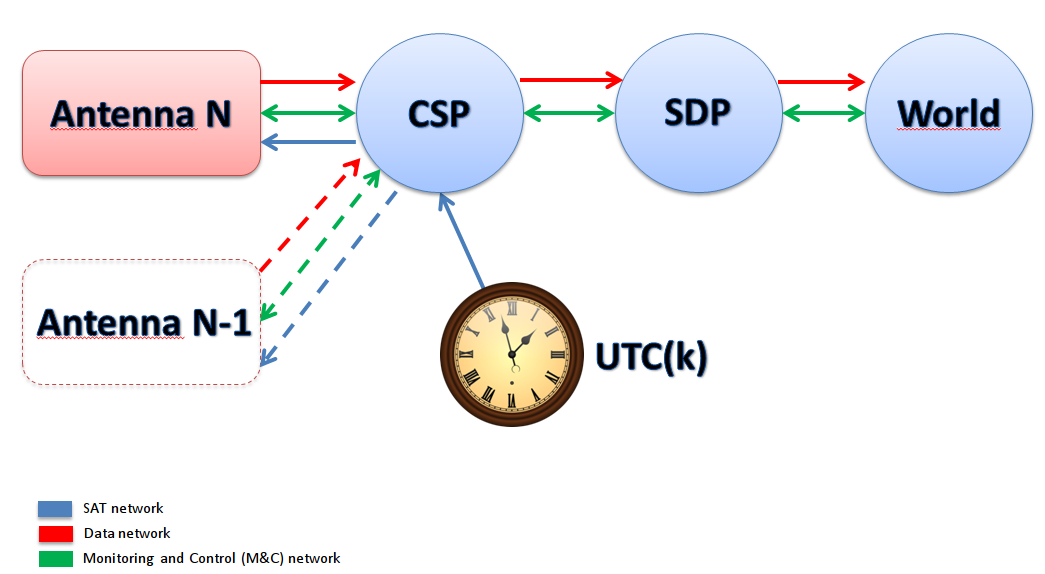
\includegraphics[scale=0.4]{img/ska_network_arch}
	\caption{The SKA Telescope network architecture is composed of three networks: the data network (red), the M\&C network (green) and the SAT network (blue). An external clock reference, UTC traceable, is provided to the whole Telescope elements in order of providing an unique time reference.}
	\label{fig:ska_net_arch1}
\end{figure}

\subsection{High-accuracy timing signals distribution for SKA1} \label{subsec:ska-distribution}

As determined by SaDT, SKA Telescope should be able to distribute a common frequency reference to all the telescopes and, in addition, provides a uniform time reference to register all the events with ultra-high accuracy through time stamps. This task is done by the Synchronization and Timing (SAT) element that belongs to SaDT. The SKA timescale is maintained by the central clock ensemble for each telescope and will be steered to within designed limits of UTC and monitored with respect to UTC via GNSS time transfer techniques. These clock ensembles form the fundamental timescale for SKA and will be the basis for precision measurements of pulsars and other time-dependent phenomenas. As consequence, during this distribution, UTC refers to UTC (SKA), as realized by the central SKA clock ensemble.
This article focuses on the solutions to distribute the UTC time by means of PPS. This PPS signal guarantees that all the scientific data are time-tag using a common reference. This time reference has high requirements coming from science that are not mandatory by other elements of the SKA systems as the monitor and control network. For these other elements, standard time transfer protocols as NTP or IEEE-1588 are a feasible solution. For the Telescope core, we illustrate that the high performance requirements imposed by the challenging scientific goals force to provide much more sophisticated approaches. 
The PPS distribution system will be in charge to deliver its output at the following locations: SKA1-MID with 133 dishes connected to optical fibre links between 120-150 km and SKA1-LOW wit 45 stations along 3 spiral arms connected to optical fibre links between 70-80 km.

Note that if the offset frequency scheme is to be applied to all SKA1-MID dishes, an additional 64 endpoints will be needed in SKA1-MID. This provides between 182 and 246 endpoints to synchronize. 
The general array SAT requirements for the frequency distribution is 1 ps while the time synchronization and time-stamp requirement is 10 ns. SaDT uses different mechanisms for achieving goals, frequency dissemination and PPS distribution. As consequence, because the goal in this contribution is just describing a solution for PPS distribution, the contribution work only considers the second requirement, the 10 ns synchronization as needed for example for the long-term timing Pulsar studies. Note that a complete description of the SKA network elements and topology is out of the scope of this contribution and only the requirements needed are presented to properly understand the need of the solution here developed. 
It is important to remark than the 10 ns requirement is allocated for the whole 
network. Because elements such as main clock also consume part of this, it 
translates into PPS-distribution time requirement of 5 ns. The error here 
includes PPS distribution, delay center precision, Dish timing transport and 
time-stamping errors and should be distributed on the different elements of the 
system that rely on the network topology that determine the number of hops. 
Based on current SAT network topology, the target specification for the 
elements of the PPS distribution system provides them an average time better 
than 2 ns. This is a quite challenging goal not only because impose a high 
accuracy synchronization goal but especially having into account the 
installation environmental conditions. The SKA1 use aerial optical fiber 
networks that are significantly affected by the large temperature excursion 
during operation, more than 20º due to the installation on desert locations of 
Sud-Africa and Australia. Furthermore the outdoor wind velocities during normal 
operation could achieve up to 40 km/h. it makes the fibers oscillate, changing 
their length, which must be compensated on real-time during execution or 
averaged them out. 

Next section will provide the description of the solution proposed to be use on SKA Telescope as mechanism for PPS distribution. 




\section{The White Rabbit synchronisation protocol} \label{sec:wr}

The WR technology \cite{Wlostowski2011} is an international collaborative
project started at CERN in 2009, later joined by other worldwide laboratories and companies. It was born as a replacement technology for CERN's accelerator timing system, but due to its versatility and improved performance compared to other alternatives, together with its open nature, it was quickly adopted by other scientific institutions. In addition to the scientific applications, some private companies such as Seven Solutions or Creotech are interested in extendind WR for industrial solutions. Some examples of that effort are the projects WR-SYNTEF \cite{web:creotech_projects} and IFMIF/EVEDA \cite{web:seven_projects}. 
Furthermore, from its very early stages, WR was launched as an open SW/HW initiative with available online sources at CERN's Open Hardware Repository (OHWR) \cite{ohwr:repo}. This encouraged different companies and research institutions to openly collaborate in its development.

The WR protocol extends PTPv2 with extra messages and has been proposed to be
included in the new PTP release (PTPv3) as High Accuracy (HA) profile
\cite{wr:maciej-ptpv3-standard} . Its main goal is to provide a synchronisation
accuracy better than 1 ns and precision in the scale of ps. The major
improvements introduced by the WR protocol address weak aspects of the PTPv2:
the limitation of the phase difference measurements to one period of the system
clock; and the assumption of symmetry between transmission and reception
paths. It inherently performs self-calibration over optical fibre links and it
is capable of distributing time to a very large number of devices with very
small degradation. Nevertheless, this technology was not designed originally
to address synchronization over long distance links, neither the inclusion of monitoring and dependable mechanisms on the nodes. Although SKA is working on improving both issues, this contribution particularly presents a new platform capable of disseminating the PPS signal incorporating flexibility and dependability features. 

The WR synchronisation mechanisms include the following elements:

\begin{itemize}
	
	\item Frequency synchronisation (syntonization): The recovered clock from the physical layer (L1) of the Open Systems Interconnection model (OSI) is used by 
	the WR logic to syntonize the local oscillator. That means that all the WR network run syntonized with the main clock reference.
	
	\item Phase synchronisation: Thanks to the syntonization, the one-cicle time resolution limitation is resolved via the use of the Dual Mixed Time Difference method (DMTD). A digital implementation of that \ref{Moreira2011} is used to achieve sub-picosecond resolution when measuring phase difference between the local oscillator and the recovered one from the upwards node.
	
	\item Time synchronisation: It is implemented by an enhanced version of the PTPv2 protocol and provides a global notion of time to the entire network. WR 
	also takes into account the asymmetries in the propagation time due to the utilisation of different wavelengths in the same fibre link improving the 
	accuracy of standard PTP protocol. 
\end{itemize}

WR implements mechanisms to ensure deterministic and reliable data transfer between thousand of nodes connected over optical fibre links up to 10 km.
However, it can easily be extended up to 50 km without significant degradation and up to 120 km without the needs of optical amplification. One application of the WR for long links can be found in \cite{Kaur2017}.

\subsection{Network topology} \label{subsec:wr-net}

A typical WR network presents a tree topology and is composed of three different
kind of elements: a Grandmaster (GM), several intermediate devices such as
switches, and end-nodes as shown in the Figure \ref{fig:wr_hierarchy}. The GM
is normally connected to a very stable clock such as an atomic clock or a GPS
receiver \cite{Daniluk2012}. The intermediate levels of the network disseminate
the timing packets to the final nodes, which are composed of other devices such
as WR Switches, WR-ZENs, WR Light Embedded Nodes (WR-LEN) or The Simple PCIe FPGA Mezzannine Card (FMC) carrier (SPEC). These devices have several ports and can behave as PTPv2 Boundary Clocks (BC). Moreover, they are connected using the master-slave scheme: some ports act as slave (upstream) of the to the upper layer while the others are masters (downstreams) and they are in charge of propagating the synchronisation to the next level of the hierarchy. The nodes of the last level of the network are known as slave devices. They recover the clock reference from the link and synchronise their local oscillators in order to provide a time reference for a specific application.

In addition to the conventional tree topology of the timing networks, new
network topologies are currently under-study in WR to add some mechanisms to improve fault
tolerance and security. Examples of this research are
\cite{jlgutierrez-paper-redundancy} and \cite{jlgutierrezhsr} that incorporate Transparent Clocks
(TC) and redundancy protocols to the WR technology such as
High-availability Seamless Redundancy (HSR) to ensure data delivery and reception in critical applications such as
control network, real-time applications or Smart Grids among others.

\begin{figure}[H] \centering 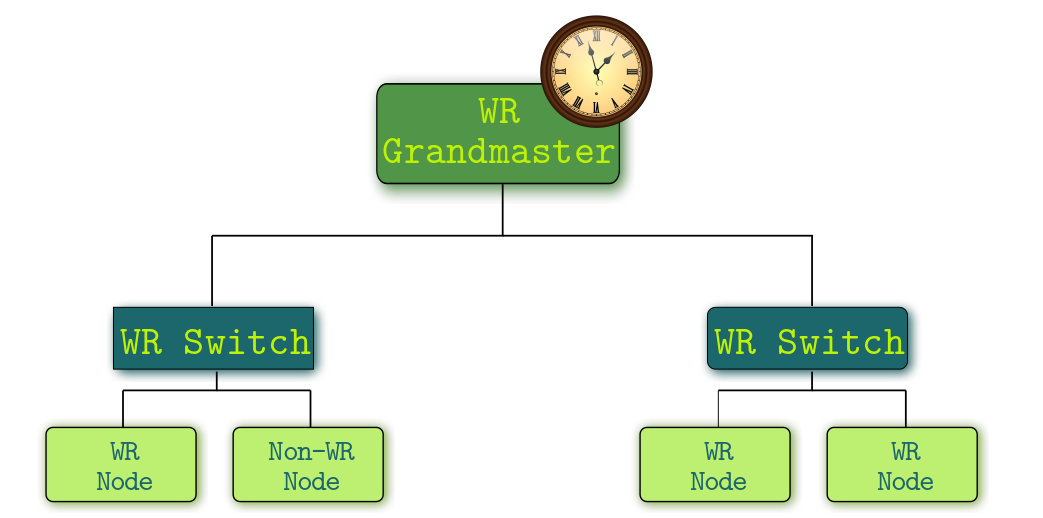
\includegraphics[scale=0.4]{img/wr_hierarchy}
	\caption{The WR network is a tree hierarchy where the root node is the
	GM that is responsible for distributing the reference time signals. The intermediate elements are WRS that acts as Gigabit Ethernet switches and as Boundary Clocks propagating the time signals from the upper layers of the network. Finally, the main purpose of the end-nodes
	is to provide timing to another specific application.}
\label{fig:wr_hierarchy} \end{figure}

\subsection{WR devices survey for the SKA Telescope} \label{subsec:wr-dev}

Regardless of the case of use for the WR technology, it will be needed to select
a suitable set of WR devices. Most applications distinguish between two main roles
according to a typical WR network: devices which act as BC, and those that act as
Ordinary Clocks (OC). Currently, the WRS \cite{ohwr:wrs} is the most convenient
BC among all the WR devices. 

The WRS has a total of 18 Small Form-factor Pluggable (SFP) transceivers, one of which can be configured as slave (upstream) and the rest as masters (downstream). It is also important to remark another I/O ports such as: five coaxial RF connectors and one management Ethernet RJ45 connector. Although there are other WR devices that could act as BC, the WRS is the most appropriate for a network with a high number of nodes, such as is the SKA Telescope, because of its high number of SFP slots.

Nowadays, there  are several WR platforms that can act as OCs. 
For this reason, we have analysed three devices taking into account the specific requirements of the SKA project.

Table \ref{tab:wr_devcomp} contains a comparison between the following three WR
devices: 

\begin{itemize} 
	\item The SPEC \cite{ohwr:spec} is a WR-compliant FMC carrier that supports low pin count (LPC) boards. It includes a Xilinx's Spartan-6 FPGA, a SFP connector and a PCIe interface. It could be used in standalone mode \cite{migueljl-paper-wr-spec}, but due to its limited computational resources, the SPEC is usually used connected to a host PC using the PCIe interface.  No coaxial RF connectors are included in this board, being this fact a major penalty since a FMC board is required to retrieve the PPS signal.
	
	\item The WR Light Embedded Node (LEN) \cite{sevensols:wr_len} is a 	standalone WR node whose main design principles are: an easiness of use and a good timing performance. It was the first WR node	that included the extended version of the WR PTP core (WRPC)architecture, the WR PTP Core Dual Port (WRC2P) \cite{torres2016scalability}. Besides the second WR-compliant Ethernet interface, the WR-LEN includes three coaxial RF
	connectors and a Ethernet RJ45 management port. Its design is quite similar to the SPEC board with some component upgrades, such as the FPGA (Xilinx's Artix-7). This device can act as BC and OC.
	
	\item The WR Zynq Embedded Node (ZEN) \cite{sevensols:wr_zen} is another
	standalone WR node but with many improvements compared to the rest of WR nodes. As in the WR-LEN, the WR implementation corresponds to the WRC2P.  This enables a BC configuration as well as OC, or GM configurations. Design is based on a Xilinx FPGA-SoC (Zynq-7000). It includes a dual ARM core included that enables the utilisation of a Linux-like	OS. The board main I/O connectors are: a FMC high pin count (HPC), two SFPs, five coaxial RF and two Ethernet RJ45. The clocking resources include a low-noise oscillator and a flexible PLL schema.
\end{itemize}

 \begin{threeparttable}\centering \ra{1.1} \begin{tabular}{@{} lccc@{}}%\toprule
	 & \rotatebox[origin=c]{60}{SPEC} & \rotatebox[origin=c]{60}{WR-LEN}  &
	 \rotatebox[origin=c]{60}{WR-ZEN} \\ \midrule \textbf{WR-compliant}\\
	 \tab\small{+BC} & \Circle & \CIRCLE & \CIRCLE \\ \tab\small{+OC} &
	 \CIRCLE & \CIRCLE & \CIRCLE \\ \tab\small{+GM} & \LEFTcircle &
	 \LEFTcircle & \CIRCLE \\ \tab\small{+Standalone} & \LEFTcircle &
	 \CIRCLE & \CIRCLE \\
		
		\textbf{RF interfacing}\\ \tab\small{+PPS output} & \LEFTcircle
		& \CIRCLE & \CIRCLE \\ \tab\small{+RF I/O} & \Circle & \CIRCLE &
		\CIRCLE \\ \tab\small{+GM input} & \LEFTcircle & \LEFTcircle &
		\CIRCLE \\
		
		\textbf{Dev. support}\\ \tab\small{+Monitoring support} &
		\LEFTcircle & \LEFTcircle & \CIRCLE  \\ \tab\small{+Linux OS} &
		\Circle & \Circle & \CIRCLE \\ \tab\small{+Available resources}
		& \LEFTcircle & \Circle & \CIRCLE \\
		
		\textbf{Extensions}\\ \tab\small{+FMC connector} & \LEFTcircle &
 \Circle & \CIRCLE \\ \tab\small{+Redundancy} & \Circle & \LEFTcircle &
 \LEFTcircle \\ \bottomrule \end{tabular} \begin{tablenotes} \item \hfill
		 \small{\CIRCLE Fully supported; \LEFTcircle Partially
 supported; \Circle Not supported} \end{tablenotes} \caption{Comparison between
 three WR nodes.} \label{tab:wr_devcomp} \end{threeparttable}

Among other WR nodes, the WR-ZEN has been the chosen development platform for the
SKA Telescope PPS system due to its flexibility and main features. The possibility of being used as a standalone node
with Linux support, the inclusion of enough I/O ports (RF, FMC, etc.), together with an improved clocking resources
looks to fulfil the timing requirements of the project.

Next section describes the proposed PPS distribution system for SKA Telescope.

\section{The PPS distribution system for SKA} \label{sec:ska-pps-system}

%% ---------------- From WR-ZEN article (EFTF2016) ------------------------
%
%The WR-ZEN is a new kind of WR node that incorporates
%a FPGA device and a hard ARM dual core microprocessor
%inside the same chip. The ARM is able to run a Linux kernel
%and this eliminates the need to use a conventional PC with an
%operating system. The flexibility of the platform has motivated
%that WR-ZEN is under study to be used in important scientific
%infrastructures such as Square Kilometer Array [11] (SKA)
%and Cherenkov Telescope Array [12] (CTA) among others.
%
%% ------------------------------------------------------------------------

The WR protocol requires a network topology similar to the ITU-T G.8275.1/Y.1369.1 standard \textcolor{red}{[REF]}, a IEEE-1588v2 telecommunication profile that describes a time-aware network capable to provide full timing support \cite{itu:TG8275_1_Y_1369_1} as explained in previous section. It uses a master time reference (SKA1 clock) that is distributed following a tree topology in a master-slave configuration. The SKA PPS distribution system is composed of two different kinds of devices: 

\begin{itemize}
	\item {The WR Switches \cite{sevensols:wr_switch}. They are standard 1U height rack-mounted equipment with 18 SFP ports and are placed in the CSPs at each of the clock ensembles. For SKA1-MID, one is placed halfway along each of the 3 spiral arms to regenerate the signal for the longest links.}
	\item{The end-nodes. They consist of a WR-ZEN node \cite{sevensols:wr_zen} powered by a Zynq FPGA-SoC and placed on inside a 1U rack enclosure. They will be located at the cores of SKA1-LOW and SKA1-SURVEY, along their spiral arms, one for each SKA1-MID dish and one for each CSP.}
\end{itemize}

The WR switches are responsible for generating the WR timing signal from the SAT clock ensembles. They lock to an external 10MHz reference and to a PPS signal, and use NTP or IRIG-B to determine the UTC time of each PPS edge. Synchronization between WR devices is performed over a a single fiber link up to 120 km using commercial SFPs.
However, the distances for SKA1-MID are longer and it is necessary to use 
intermediate WR switches as repeaters with a penalty over the system 
performance due to increment of the inherent noise of each WR device that it is 
propagated to the down-link nodes. An analysis of the jitter evolution for 
network with many hops could be read in \cite{torres2016scalability}. Thanks to 
network similarities between WR and SKA, both can use the same single fiber 
strand available for the SAT network. 

\begin{figure}[H]
	\centering
	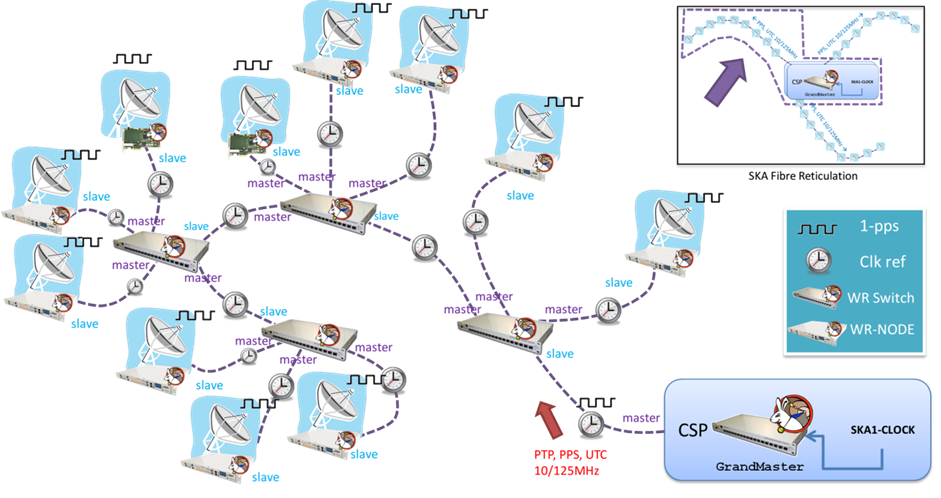
\includegraphics[scale=0.4]{img/ska_pps_network}
	\caption{Network topology for PPS signal distribution based on WR switches and nodes. The figure shows the different elements and the network topology. }
	\label{fig:ska_pps_dist_network}
\end{figure}

%\missingfigure{Example of a network topology for PPS signal distribution based on WR switches % and nodes}
 
An important feature of the system to take into account is that the PPS pulse itself at each station is derived from the reference frequency distributed from the SKA clock and not from the WR system. In normal operations, the WR system only monitors the absolute time of each PPS and reports it back activating an alert if the PPS signal does not align with the start of the UTC second. This condition indicates something is wrong in the timing chain and the station must be discard data to ensure not to introduce corrupt one in the system. Other functionality associated with the WR part is to temporarily alter the division ratio to bring the PPS edge back in alignment with UTC time. In this case, fringe finding must then be performed to restore full calibration again.

The centrally located WR switches and the WR end-nodes are connected to by a 
single strand of single-mode fiber with LC/PC connectors and industry standard 
bi-directional SFPs that use two wavelengths (down-link and up-link) to produce 
optical signals to be transmitted. Finally the end nodes generate a 1PPS signal available. 

As previously described, this solution requires WR switches and nodes. The former are well-defined equipment with known interfaces and software support. 

For the implementation of the SKA nodes, we have proposed the utilization of the WR-ZEN board. Thanks to this new platform, the utilization of a host computer/crate to host the FPGA card can be avoided which reduces significantly the equipment price and is also a remarkable improvement in term of dependability which is a key factor taking into account that SKA Telescope should have an annual availability of about 95\% of the time (although degraded operation modes can be allowed under some circumstances).
Finally note that all these features are possible keeping the full flexibility of a complete CPU+FPGA system on a single board. 

In the following section we will describe the proposed node hardware, gateware and firmware that have been developed as a candidate solution for the SKA Telescope PPS distribution system. 

\subsection{A PPS distribution node architecture} \label{subsec:ska-pps-system-arch}

%% ------------------------ Javi ------------------------------------------
%% As a case of study, we can focus on the ZEN board that holds the Dual WRC (D-WRC), a revision from the original WRC developed by Seven Solution in our new line Xilinx 7 Series products. The D-WRC is %% able to synchronize two WR nodes or to be an intermediate link in a daisy chain network. In addition, the ZEN board includes high precision, low jitter and temperature compensated clock resources 
%% controlled by the D-WRC. Furthermore, the Dual core ARM Cortex processor, run under Linux OS, facilitating the development of user applications taking advance of the best from the WR technology and 
%% the ZEN resources. The on-board Linux allows the utilization of new and interesting features as webservices for configuration, SNMP support for status monitoring and remote firmware load and update. 
%% ------------------------------------------------------------------------

The PPS distribution system for SKA is based on the WR-ZEN platform that provides the WR support in order to ensure the synchronization accuracy in the system. The first design of the PPS system includes the Fine Delay FMC card that is used to generate the timing signals through mezzanine channels and has two Network Interface Cores (NIC) that allows accessing optical fiber ports as conventional Linux network interfaces. An introduction to this platform is presented in \cite{migueljl-paper-wr-zen-intro} and a contribution that improves the NIC bandwidth of the design in \cite{jorgesg-paper-wr-zen-dma}. Moreover, the WR-ZEN is also under study for other FMC cards such as the FMC ADC one to build a distributed oscilloscope \cite{joselj-paper-wr-zen-adc}.

Nowadays, the utilization of the Fine Delay FMC card is still under discussion and there is a possible design whose its final architecture could be addressed without this module.

\subsubsection{Hardware}
\label{subsec:hardware}

%% ---------------- From WR-ZEN article (EFTF2016) ------------------------
%
%The WR-ZEN is a small stand-alone board that integrates
%the latest Xilinx Zynq Z-7015 device with a Dual ARM
%Cortex-A9 MPCore with CoreSight and containing an Artix
%FPGA-logic with 74K logic cells, 380KB of embedded mem-
%ory and 160 DSP blocks. It has two optical SFP Ethernet
%interfaces, two copper Ethernet ports and the FMC expansion
%connector. On addition to FMC, a SAMTEC connector is
%available for developing of simple expansion boards and some
%USB sockets for monitoring. The WR-ZEN node is provided
%with improved oscillators, PLLs and a clocking scheme that
%provides significant better short term stability than previous
%WR node designs. It also includes several SMA outputs that
%can be configured to generate signals from the FPGA and an
%input that allows the WR-ZEN to behave as grandmaster. The
%WR-ZEN can be used with several FMC cards depending on
%the application: ADC, DAC, TDC, DDS, Fine delay, Digital
%I/O, etc.
%
%% ------------------------------------------------------------------------

%% ------------------------ Javi ------------------------------------------
%%The ZEN board is intended to be a high precise time provider and offers a large amount of possibilities facilitated by diverse connections and expansions:
%% - IRIG-B I/O: This is the Time of Day used by the ZEN board. It is able to work as master or slave.
%%- Two 10/100/1000 Ethernet ports connected to the ARM processors that can be used for diverse network applications and protocols (NTP, sNTP, PTPv2, management, etc..).
%% -Two SFP Cages where the WR compliant links are plugged.
%% -SMA connectors to enable the ZEN to synchronize itself with more precise clocks, e.g. GPS source or high stable oscillators, or providing a diverse set of clocks synchronized by WR.
%% - FMC connector to plug one of the mezzanine boards developed in the framework of the WR project or any other industrial one existing in the market. These FMC cards enhance the possibilities of the %%ZEN; e. g. FMC-ADC, FMC-DIO, FMC-FineDelay, FMC-DAC, etc; and allows many products configurations. 
%% - Memory resources; SD, DDR3, Flash.
%% - Two UART-USB connectors; for management and debugging in the D-WRC and Cortex processors.
%%In brief, the ZEN board offers to the final user a node capable to reach sub-nanosecond synchronization, working in daisy chain schemes, and provides the best of the Zynq and its new level of system %%design capabilities.
%% ------------------------------------------------------------------------

The WR-ZEN board is a proprietary design of the Seven Solutions company 
developed in 2015. The major design changes respect to previous designs for 
WR-nodes are the inclusion of a Zynq FPGA-SoC platform from Xilinx, and a 
flexible clocking scheme. The former, enables a more structured design where 
the software can be organized in abstraction layers. This is achieved by the 
inclusion of an Linux-like OS and many low-level drivers and a Hardware 
Abstraction Layer (HAL) whose most important result is an easy and quick 
development of new functionalities on top of all the software that interfaces 
with the underlying hardware. A deeper detailing of the software structure is 
given at subsection \ref{subsec:software}. The latter, makes the new board 
suitable for many synchronization applications with diverse requirements.

\begin{figure}[H]
	\centering
	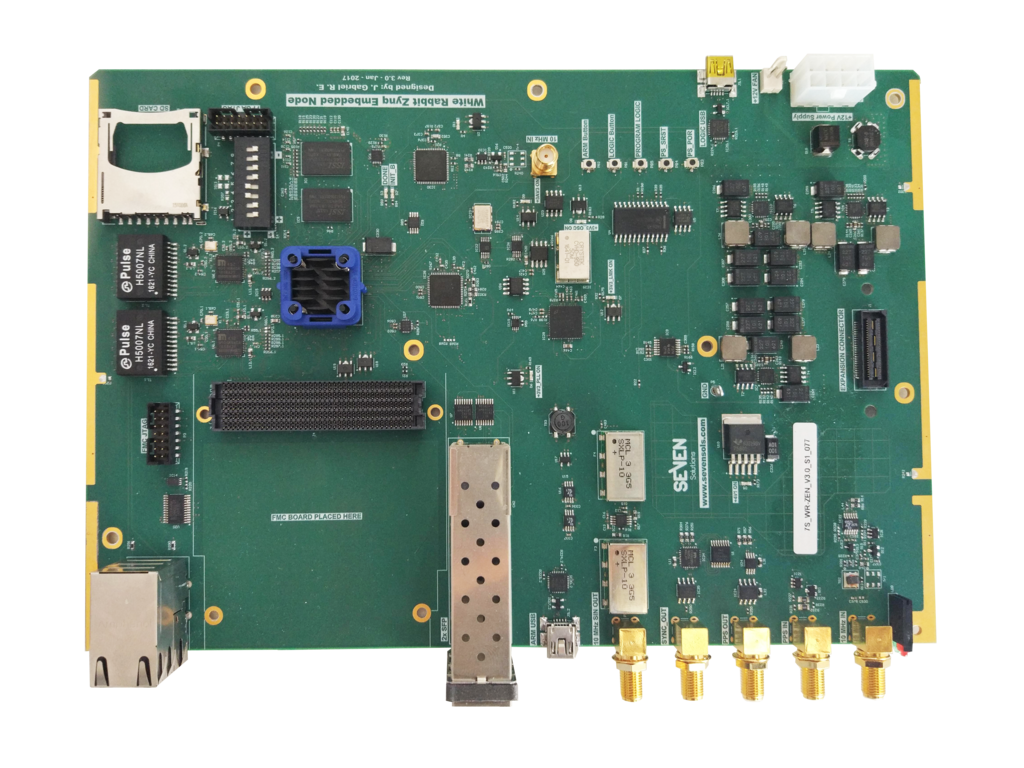
\includegraphics[width=0.7\linewidth]{img/wrzenv3_scaled}
	\caption[WR-ZEN board picture]{The picture shows the WR-ZEN board with the 
	FMC Fine Delay connected. Main connectors are shown: Ethernet ports, SFP 
	ports and the SMA connectors for the RF input/output signals.}
	\label{fig:wrzen}
\end{figure}

The FPGA-SoC platform breaks up design in two different parts: (i) the 
Programmable Logic (PL) including modules described in HDL; and (ii) the 
Processing System (PS) formed by all the software executed by the ARM processor.
The inclusion of a hard-processor is something new in the node architecture. 
Previous designs argued for a simple and cost-effective design where software 
code was executed in an embedded-processor \textcolor{red}{[REF]}. But the adoption of the WR 
technology by other scientific and industrial entities stated the lack of free 
system resources and a clear development process in order to host their 
customizations \textcolor{red}{[REF]}. These problems have been solved by the WR-ZEN design: a 
powerful hard-processor for software and more free resources in the FPGA side 
due to pass some of the software from the embedded-processor to the ARM. In 
addition to that, the Zynq platform includes the needed physical components by 
the WR design: internal programmable PLLs, Gigabit Transceiver Ports (GTPs), 
and other not strictly fundamental por a WR-node but which could be very 
helpful in future designs such as Ethernet interfaces with hw timestamping 
support (allowing PTPv2 support). I/O ports are also very important because 
they will interface with external components which can obtain synchronization 
from the base board. The most relevant I/O interfaces of the WR-ZEN are the FMC 
HPC socket (support for the OHWR \cite{ohwr:repo} FMC cards 
\cite{ohwr:fmc-fine-delay}), two SFPs sockets capable of BC configurations, and 
many external RF connectors for input/output of RF signals and the PPS.

\begin{figure}
	\centering
	\includegraphics[width=0.7\linewidth]{img/zenclkschema}
	\caption[WR-ZEN clocking schema]{The figure depicts the new clocking schema 
		presented in the WR-ZEN desing. The most relevant changes considering 
		previous designs are: the inclusion of an external PLL to lock an 
		external 
		stable clock reference (GrandMaster mode), and a flexible path in the 
		main 
		clocks path allowing the final user to choose between a low-noise PLL 
		and a 
		full-featured PLL with many options such as programmable output delays.}
	\label{fig:zenclkschema}
\end{figure}

The extended WR clock schema is depicted in Figure \ref{fig:zenclkschema}. 
Besides including new components, the WR-ZEN design, upgrades some of them 
looking for an increment of the clock stability. All the clock path: DAC, VCXO, 
PLL has received an upgrade. A new DAC with a better response time and 
stability, and low-noise VCXO and PLL have been included. But the PLL from 
previous designs is maintained because it offers some key aspects such as 
programmable output delays. To avoid cascading many PLLs, the signal from the 
XO is droved to the low-noise PLL first because it allows bypassing its 
reference to other components without adding noise to the reference. This 
schema enables using both PLLs at the same time. One of them is used to 
generate all the WR-clocks and the other could be used to generate custom 
frequencies not available from the other for example. The WR general 
performance is limited by the noise when locking to an external reference, in 
the so called GranMaster mode, described in \cite{Rizzi2016}. The conclusion of 
that contribution is that in order to decrease the noise when locking to an 
external reference, internal PLLs in the FPGA should be avoid. Instead of it, 
it is recommended an Analog external PLL which locks to the external reference 
and generated the needed clock signal by the internal elements of the WR-logic 
in the FPGA. That results are included in the version 3.0 of the WR-ZEN as 
shown in Figure \ref{fig:zenclkschema} looking to achieve the expected PPS 
distribution stability requirements of the SKA project.


\subsubsection{Gateware}
\label{subsec:gateware}

%% ---------------- From WR-ZEN article (EFTF2016) ------------------------
%
%The gateware refers to the design that must be programmed
%in the Programmable Logic (PL) and the Processing system
%(PS) configuration to be applied. The PL is based on the Wish-
%bone (WB) bus [13] and has a main crossbar that interconnects
%the different IP cores.
%In the Fig. 2, the PL architecture is represented in more
%detail.
%* GIGABIT TRANSCEIVER PORTS (GTP): These
%blocks contain primitives to transfer data through a
%high performance dedicated interfaces. The GTPs are
%connected to the SFP sockets and allow to send/receive
%packets to/from the Gigabit Ethernet network.
%* WR PTP DUAL PORT CORE (WRPC-2P): It is the
%key core for WR nodes and contains all the elements
%needed to implement the WR protocol for two optical
%fiber ports.
%* AXI TO WB BRIDGE (AXI-WB BRIDGE): The PS
%must be able to talk to the PL. However, the PS
%uses the AMBA/AXI bus specification instead of the
%WB one of the PL. The AXI-WB bridge is able to
%convert from WB transactions to AXI transactions and
%viceversa.
%* FMC CORE: This IP core gives the specific function-
%alities for a certain kind of FMC card. In the reference
%design, the Fine Delay FMC core is included.
%* NETWORK INTERFACE CORE (NIC): It provides a
%network controller that is directly accesible from the
%Linux kernel. The NIC module can be managed like a
%standard network interface thanks to a specific driver.
%The gateware design carries out a WR compliant node
%with network capabilities and support for several FMC cards.
%However, the reference design only uses the Fine Delay FMC
%card, it can be extended easily to work with other cards such
%as DIO, TDC, ADC, etc.
%
%% ------------------------------------------------------------------------

The designed gateware (FPGA firmware) is built on two different levels. The former uses the AMBA bus specification and considers the main elements for the Zynq ecosystem with several components such as Zynq Processing subsystem that takes care of configuring the ARM microprocessor and controlling the bus interconnections with it, a reset and clocking module that manages the clock and reset signals, an AXI QSPI core to program the hardware PLL chip, an AXI crossbar to glue everything together and a specific IP core that represents the next level of the design that is explained in following lines.
\textcolor{red}{[muy tocho, hay que reescribirlo con frases más cortas]}

The design (shown in the Fig. \ref{fig:gateware_first_level}) is based on AXI and WB buses and has several crossbar modules to interconnect
all the components. Due to the different buses, there is an AXI-WB bridge that is responsible 
for converting AXI transactions into WB ones. This is necessary because the Zynq Processing System 
uses the AXI protocol but most WR compliant modules are based on Open Core WB bus. The WR Dual Port 
core implements the WR functionalities for the WR node. The main components of the WR Dual port core 
are the LM32 soft-microprocessor that runs a specific firmware with WR functions stored in the WB RAM, 
a WR endpoint that is charge of network transmissions/receptions over a 1 Gigabit Ethernet link, 
the WB PPSgen core that contains the timebase counter for the WR technology and the SoftPLL
that controls the servo loop algorithm to follow the master clock. The GT transceiver is a Xilinx primitive
that allows to implement high speed interfaces such as 1 Gigabit Ethernet links. The NIC cores are responsible
for receiving/sending packets between the ARM microprocessor and the network. The TxTSU module is a conventional
FIFO designed to store the transmission timestamps of the sent packets in order to give some time to the driver to
access them. The Fine Delay FMC core is a controller for the Fine Delay FMC mezzanine card. The main task for this 
board is to configure a delay to transmit a signal from the TTL trigger buffer to one of its four outputs.

%\missingfigure{Add figure to show first level architecture.}

\begin{figure}[H]
	\centering
	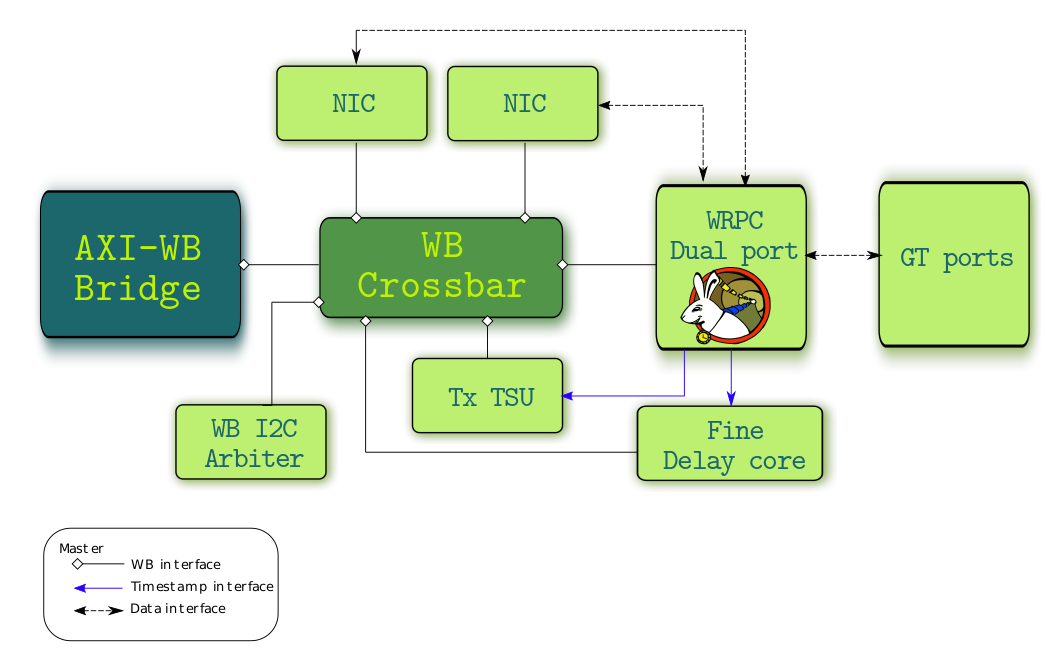
\includegraphics[scale=0.4]{img/gateware_first_level}
	\caption{Gateware project design. The figure shows the main components of the design. The most important one is the WRPC dual port that is responsible for implementing the WR protocol. The Gigabit Transceiver ports allows to transmit/receive packets to/from the network through the optical SFP modules. The NIC cores manage Ethernet packets and behave as standard network interface cards for the ARM microprocessor. The AXI-WB Bridge translates AXI transactions into WB ones. It is important because the ARM is connected using AMBA specification meanwhile the WR FPGA cores use Wishbone bus standard. Finally, the Fine Delay core contains the resources needed to control the Fine Delay FMC card.}
	\label{fig:gateware_first_level}
\end{figure}

The second level is referred to the specific IP core that takes into 
consideration the WR protocol and other basic features such as Gigabit 
networking, serial debug communication, timestamp mechanism, etc. This module 
uses the Wishbone Open Cores bus specification and is mainly 
vendor-independent. It is composed of many IP cores that are interconnected 
through a WB crossbar that allows bidirectional communication between any two 
IP cores. Moreover, the crossbar can store Self Descriptor Bus (SDB) 
information about the different components attached to it in order to discover 
them with a scan operation. Thanks to it, the WB peripherals can be discovered 
automatically by software tools and this allows not to hard-code the different 
addresses inside the source code improving the maintainability of the system. 

\textcolor{red}{[esta sección tiene demasiados detalles de ingeniería que hacen perder el hilo de lo que se está intentando conseguir. Hay que ser muy claro diciendo cómo es el gateware y qué funcionalidad tiene pero creo que hay detalles que se pueden obviar.]}

\subsubsection{Firmware} \label{subsec:firmware}

The firmware code is related to all the functionalities needed by the WR protocol. In the node architecture, the embedded software part of the WR 
protocol and some device drivers runs in the soft-microprocessor describe in 
the previous section. The main tasks of the WR routines are the servo 
loop algorithm which, maintains the lock to the recovered frequency from the 
master device, and the implementation of the WR-PTP stack. In addition, a 
simple Command Language Interface (CLI) is introduced to allow 
the user interaction \textcolor{red}{esto es demasiado informal: (think that some WR nodes can work in standalone mode and 
does not have an on-board hard microprocessor)}.

\subsubsection{Software} \label{subsec:software}

%% ---------------- From WR-ZEN article (EFTF2016) ------------------------
%
%In this section, the software components needed to run a
%Linux kernel/Baremetal application on the WR-ZEN board are
%described. The Zynq devices needs a binary file (BOOT.bin)
%that is composed of a specific Xilinx bootloader known as First
%Stage Bootloader (FSBL), a gateware bitstream to program
%the FPGA and a baremetal application or a Second Stage
%Bootloader (SSBL) if Linux kernel must be loaded. The FSBL
%is encharged to initialize different peripherals, configure the
%FPGA with a bitstream and run the baremetal application
%or the SSBL. The baremetal application is encouraged to be
%coded with the Xilinx SDK because all the gateware details
%are imported to the software project and we can use all the
%functionalities of the Xilinx Board Package Support (BSP). On
%the other hand, the SSBL is a independent project and must be
%downloaded and compiled separately. The most common SSBL
%are U-boot [14] and Barebox [15]. The chosen bootloader is U-
%boot instead of Barebox because there is a Xilinx repository
%[16] that includes custom code for the Zynq devices. When
%everything is generated, the Xilinx SDK or bootgen tool must
%be used to pack all the binaries in a single file, the BOOT.bin.
%The following step is to compile the Linux kernel, kernel
%modules, libraries and userspace tools. To face this task, there
%are two ways. The first one is to compile every component
%separately and manually. It is very slow, tedious and error
%prone but it is the best way to control the different steps
%and customize them if necessary. On the other hand, there
%are some tools that automate the process such as Yocto [17]
%or Buildroot [18]. However, they present a disadvantage: the
%user loses the control and it is more difficult to add some mod-
%ifications because the tool does everything automatically. For
%the reference design, the Buildroot is used to ease and speed
%up the compilation of the Linux kernel, U-boot bootloader, the
%kernel modules and userspace tools. The Buildroot package is
%retrived from the official project website. It is very configurable
%and includes the Kconfig support to enable/disable the different
%features similar to the Linux kernel. Although the Buildroot
%eases very much the compilation process, it has many options
%and may be confusing for a non-expert user. To solve this
%issue, a set of scripts have been implemented to perform all
%the actions needed and configuration files for the Busybox,
%Linux kernel and the Buildroot are provided. This scripts are
%based on others from the WR Switch Software project [19] of
%the OHWR repository.
%In addition of the Linux kernel and the bootloader, some
%kernel modules and userspace tools for the WR-ZEN board
%have been written. The main kernel driver is the WR-ZEN
%carrier, known as zen, and is responsible for reprogramming
%the FPGA device and reading the EEPROM information of
%the WR-ZEN board. This driver is based on the fmc-bus
%[20] (OHWR) and it also gives NIC capabilities to manage
%the optical fiber ports as standard network interfaces from
%the Linux kernel. Some userspace tools to read/write the
%FPGA register (zenmem), reprogram the FPGA bitstrean (zen-
%fwloader.sh), reprogram the soft-microprocessor program (zen-
%cl) and send commands to the soft-microprocessor (zen-vuart)
%are included too. The driver and all these tools are inspired by
%the SPEC Software project [21] of the OHWR repository. As
%we saw in the previous section, the reference design has also
%a Fine Delay core that must be controlled by a specific kernel
%driver. Actually, there are two drivers (zio [22] and fmc-fine-
%delay [23]) and some userspace tools in the OHWR for the
%Fine Delay FMC card in a SPEC card. Using these ones as
%starting point, some minor modifications have been made to
%incorporated them to the WR-ZEN reference design.
%
%% ------------------------------------------------------------------------

The WR-ZEN is the first WR node taking advantage of a Linux 
based operative system (OS). Due to the inclusion of a dual-core ARM 
microprocessor in the platform, the system design is not longer tied to 
low-level software design. New functionalities, such as communication 
protocols, management tools, etc., are quickly added because of the 
facilities \textcolor{red}{facilities???} of an OS: a hardware abstraction layer, and drivers which abstract 
the management of the underlaying logic. This middleware adds also more 
security controlling the access to the hardware.

The counterpart is an increment in the complexity of the system design. The new platform takes advantage of its hard dual core microprocessor to deploy a Linux system or a standalone application.

In the SKA system, the WR-ZEN is used with a Linux 
kernel to ease the implementation of the specific applications and providing 
conventional mechanisms to add more functionalities and update the entire 
system in a fast and ease way which is not included in the current WR node 
embedded design \textcolor{red}{info duplicada}. In order to build all the software components, some custom 
scripts (inspired by WR Switch Software project ones from OHWR) are added to 
allow user intervention and provides standard configuration for Linux kernel, 
Busybox and root filesystem.  
Moreover the basic Linux components, some userspace tools and custom kernel 
drivers have been developed to manage the main modules in the WR-ZEN reference 
design. The FMC kernel driver (\textbf{fmc}) is retrived from OHWR repository and it has not
been modified. Its main purpose is to implement a generic support for FMC bus
in the Linux kernel. The main driver for the WR-ZEN platform is the \textbf{zen} one
and manages all the IP cores in the design, create standard Linux network interfaces and
reprogram the FPGA with the proper bitstream. The \textbf{zio} driver is 
retrieved from OHWR
repository and it has not been modified. It creates the ZIO bus that exports driver attributes
through the SysFS. The \textbf{fmc-fine-del} module implements the Fine Delay FMC functions and
it is based on the OHWR repository one but includes some modifications to work properly in the
WR-ZEN platform. The \textbf{zen-nic} driver is responsible to enable/disable the network 
interface methods of the \textbf{zen} module.

As previously seen, there are dependencies between the different kernel drivers and it establishes the installation order. The \textit{zen} one depends on \textit{fmc}. The \textit{fmc-fine-del} needs \textit{zen}, \textit{zio} and \textit{fmc}. The \textit{zen-nic} only uses the \textit{zen}.

In addition to device drivers, there are several custom userspace tools related with drivers previous explained. Those that use the \textit{zen} driver API are \textit{zenmem} that is responsible for accessing memory map of the WR-ZEN IP cores, \textit{zen-fwloader} that programs the FPGA with a given bitstream, \textit{zen-vuart} and \textit{zen-cl} that allows talking to the soft-microprocessor (see the gateware section) and loading other firmware respectively. On the other hand, the  \textit{fmc-fine-del} driver has associated tools such as \textit{fmc-fdelay-board-time} that is used to get the current time, \textit{fmc-fdelay-pulse} that generates pulses with certain characteristics (frequency, initial delay, duty cycle, etc), \textit{fmc-fdelay-input} that prints some information when an incoming signal raises the input connector of the mezzanine card, \textit{fmc-fdelay-list} that enumerates the Fine Delay FMC cards plugged in the system (only one for WR-ZEN but however more for conventional PCs), \textit{fmc-fdelay-status} that check the status of Fine Delay FMC core and \textit{fmc-fdelay-term} that configures the termination of each channel among others.

Apart from the Linux or standalone environment described before, more 
components are needed  for the WR-ZEN platform. Previously any application or 
Operating system can run, a specific bootloader must initialize some hardware 
devices. In the Zynq technology, there is a special bootloader known as First 
Stage Bootloader (FSBL) that is responsible for early initializations and it is 
the first step to perform in whatever system based on Zynq. The FSBL sets up 
different peripherals, configures the FPGA with a bitstream and runs the 
standalone application or the Second Stage Bootloader (SSBL) which finally 
loads the Linux kernel in the RAM memory and prepare the system to run the 
specific user applications.

\begin{figure}[H]
	\centering
	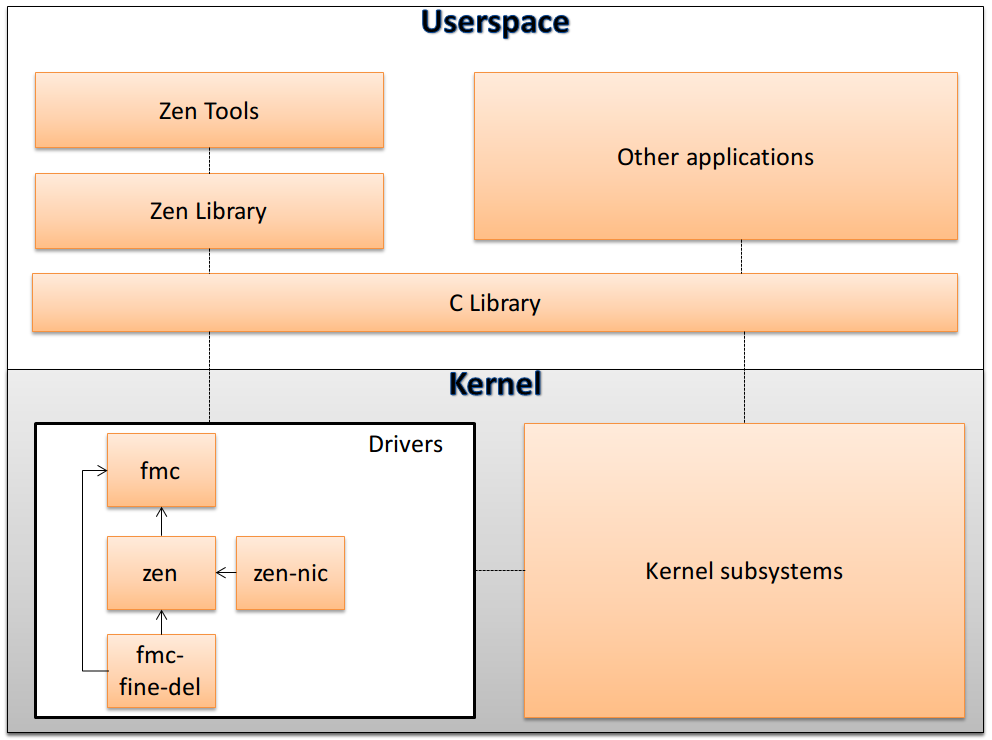
\includegraphics[scale=0.4]{img/software_architecture}
	\caption{Software architecture. The picture shows the software architecture
		used by the design. It is based on Linux kernel and several tools and drivers
		have been developed for the WR-ZEN board. The tools can be used to program 
		the FPGA, update the soft-microprocessor code or connect to the virtual UART
		interface of the WRPC-2p. They call the Zen Library procedures that finally
		use C Library functions and switch to kernel mode through system calls. In the
		kernel space, the drivers are responsible for implementing all the requested 
		functionalities. }
	\label{fig:software_architecture}
\end{figure}

\textcolor{red}{Demasiada tela. No sé hasta qué punto es interesante decir que se han hecho drivers, sus nombres, funcionalidad, el FSBL, los scripts que se usan para generar las imágenes... Esto no es para un artículo. Tenéis la imagen, hablad sobre ella, lo que está fuera de ella que no sea relevante, se debería quitar.}

\textcolor{red}{lo siguiente son los experimentos, falta hilo conductor}



\section{Experiments \& results} \label{sec:experiments}

%% Section that includes the experiments performed.

This section describes the accomplished experiments that prove how the developed system fulfills SKA's requirements for the PPS distribution system. The first experiment is a general characterization of the developed platform. The second one, tests the equipment in a realistic network topology to evaluate the performance in a possible deployment. The last experiments evaluates the influence of some typical events, such as traffic, temperature fluctuation or \textcolor{blue}{something else} in a network deployment using the WR-ZEN.

Performance of the new WR platform is measured using multiple equipment, and obtained results have been compared to WRS's performance because of it's electronic design is considered as reference for WR technology. The list of the equipment and materials used for the experiments is the following:

\begin{itemize}
    \item Two White Rabbit Switches to simulate a typical WR network. All of them have hardware version 3.4 and 5.0 of firmware.
    \item A White Rabbit ZEN Time Provider (WR-ZEN TP) to test the performance of the new developed platform as node of a WR network. The firmware version is 1.2.
    \item Phase noise plots, ADEV, TDEV and TIE measures have been taken using a Symmetricom 3120A.
    \item PPS stability tests have been measured with a Keysight 53230A Timer.
    \item The 3120A needs an external stable clock reference. That reference is also needed as input for the WR equipment when Grand Master mode is set. A Morion MV89 Oven Controlled Crystal Oscillator (OCXO) has been used as clock reference for the experiments.
    \item Multiple components for the setup of the equipment:
    \begin{itemize}
        \item Small form-factor pluggable transceptors (SFPs) to stablish the link between WR devices.  \textcolor{blue}{\textit{TODO:} Completar cuando se hayan usado}
        \item Optical fiber links. \textcolor{blue}{\textit{TODO:} Completar con las fibras que se hayan usado}
        \item \textcolor{blue}{\textit{TODO:} Something else?}
    \end{itemize}
    \item \textcolor{blue}{\textit{TODO:} Completar conforme se hagan medidas}
\end{itemize}

\subsection{Characterization of the WR-ZEN platform}
\label{subsec: charact_zen}

% Aquí las pruebas típicas de caracterización

The new components included in the clocking's scheme of the WR-ZEN (fig. ?), described in subsection \ref{subsec:hardware}, offer a performance improvement respect to previous WR designs, such as the WRS. 

\missingfigure{Esquema de las medidas realizadas}

The following experiments evaluate phase noise performance of the frequency transfer in WR at different scenarios: a) Grand Master mode, to evaluate how the WR-ZEN syntonizes to an external reference clock. b) Master mode, that reflects the characteristics of the new internal XO of the WR-ZEN. c) Slave mode, to see the behavior of the new design as slave node of the network. Different configurations are depicted in fig. ?? to allow the reproduction of the different experiments of this paper.

\missingfigure{testing schemas}

The Free running mode (FR) is not affected by the WR's logic, it is mostly influenced by noise of the crystal oscillator (XO). A master node is placed at top of a timing network hierarchy, and unlike a Grand Master node, it is not locked to any external reference. So that, a master node with an improved stability will benefit the performance of all the downlink devices connected to it.

Picture \ref{fig:zen_vs_wrs} shows an high jitter accumulation in low frequencies for the WRS (orange curve). Integrating noise from 1Hz to 10 Hz, we see a difference of 60.1 ps of RMS jitter between WRS and WR-ZEN. Other results can be checked in table \ref{tab:pn_results}. It is worthy to remark difference between sine wave output and TTL output in the WR-ZEN board. As detailed in fig. ?? \textit{(clock schema)} there are two 10 Mhz clock outputs in the WR-ZEN. One comes directly from the AD9516-4 PLL, the sine wave output. The other, comes from FPGA logic but it is latched using a clock signal from the LMK03806 PLL. It would be foreseeable to expect an higher jitter in the signal from the FPGA, but thanks to the low noise profile of the LMK PLL we can remove much of the jitter of that signal and decrease the floor noise of it.

\begin{figure}[t]
	\centering
	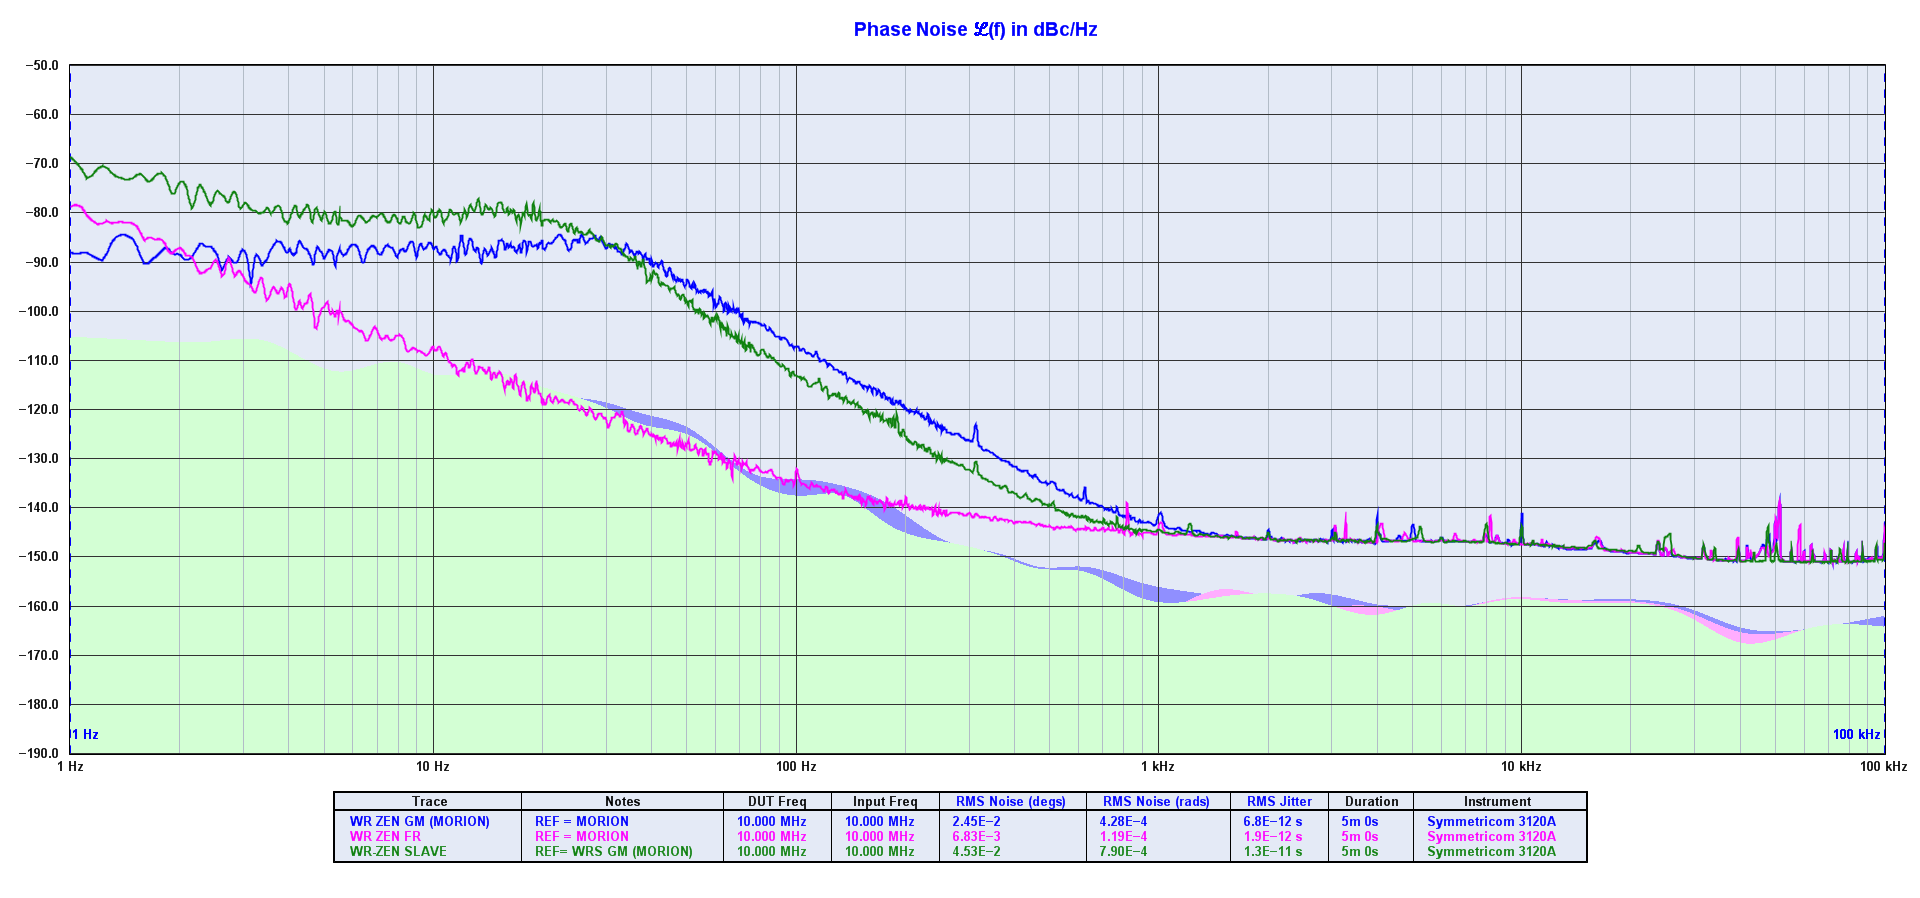
\includegraphics[width=0.8\textwidth]{../measures/img/zen_all}
	\caption[Phase noise plot of the WR-ZEN]{The figure shows the Phase noise plot for the WR-ZEN in the Grand Master, Free Running and Slave modes. Sine wave output is compared to CMOS output.}
	\label{fig:zen_pn_all}
\end{figure}

\begin{figure}[t]
	\centering
	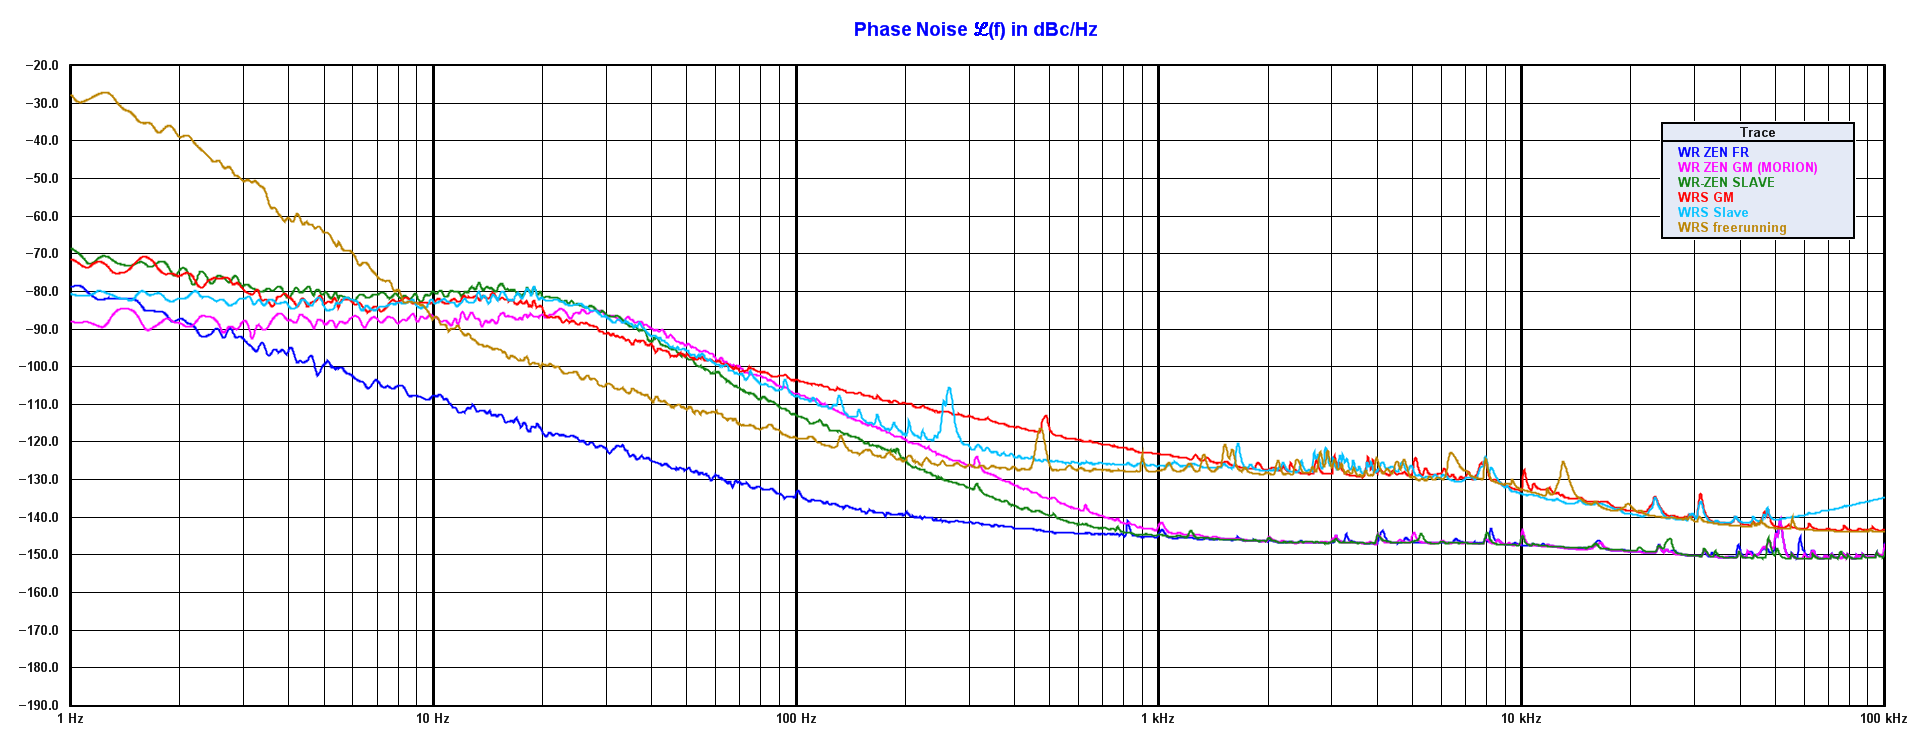
\includegraphics[width=0.8\textwidth]{../measures/img/zen_vs_wrs}
    \caption[Phase noise plot of the WR-ZEN vs WRS]{The figure includes the same phase noise measures for the WRS. In this plot, only the CMOS outputs appear because the WRS doesn't have sine wave output signals.}
    \label{fig:zen_vs_wrs}
\end{figure}

It is also relevant testing the performance of the system when locking to an external reference in Grand master mode because the board is intended to be used as Time Provider. Additive noise of the WR-ZEN will be propagated downstream, decreasing the quality of the Grand master's reference clock. It's very important that the system adds low noise in order to not degrade the quality of the external reference clock.

Results included in table \ref{tab:pn_results} and ploted in figure \ref{fig:zen_vs_wrs} unveil a jitter reduction in the WR-ZEN compared to the WRS of 2.1 ps of RMS jitter integrated from 1Hz to 100kHz. This is a relevant because jitter in the slave nodes will benefit from a noise reduction in the Grand Master node.    
    
 \begin{table*}\centering
     \ra{0.8}
     \begin{tabular}{@{} rcccc@{}}%\toprule
         & \multicolumn{4}{c}{\bfseries{RMS jitter (ps)}} \\
         \cmidrule(l){2-5}
         & 1Hz-10Hz & 10Hz-1kHz & 1kHz-100kHz  & 1Hz-100kHz \\ \midrule
         \textbf{Free running}\\
         \small{WRS (CMOS)}             & 62  & 1.7  & 1.1  & 62  \\
         \small{WR-ZEN (\textit{sine})} & 2.1 & 0.24 & 1.4  & 2.5 \\
         \small{WR-ZEN (\textit{CMOS})} & 1.9 & 0.21 & 0.26 & 1.9 \\
         \cmidrule(l){2-5}
         
         \textbf{Grand Master}\\
         \small{WRS (CMOS)}             & 7.3 & 6.7 & 1.1 & 9.9\\
         \small{WR-ZEN (\textit{CMOS})} & 2.8 & 6.2 & 0.26 & 6.8\\
         \cmidrule(l){2-5}
         
         \textbf{Slave node}\\
         \small{WRS (CMOS)}             & 4.9 & 8.2 & 1.2  & 9.7\\
         \small{WR-ZEN (\textit{CMOS})} & 8.5 & 9.3 & 0.24 & 13\\
         
         \bottomrule
        \end{tabular}
        \caption{Phase Noise results extracted from plots in figure \ref{fig:zen_pn_all} and \ref{fig:zen_vs_wrs}.}
        \label{tab:pn_results}
\end{table*}

The slave mode results show that WR-ZEN performs slightly worse than WRS. Noise between 1 Hz and 20 Hz increases the RMS Jitter of the WR-ZEN in ?? \textit{sacar de los datos en crudo!!}. The observed difference could be caused by a bad adjustment of some of the internal parameters of the control loop for the slave mode. This will be treated in future work because the scope of this contribution is characterize the initial design of the WR-ZEN.

\subsection{Network experiment} %% Buscar un nombre mejor
\label{subsec: net_exp}

The next experiment covers the analysis of timing distribution over a WR network formed by a WRS in the top of the hierarchy locked to an external reference (Grand Master), an intermediate WRS and a final node, the WR-ZEN. We planned to reproduce an example of time distribution for the SKA facilities where it won't be there so many hops between the clock reference and end nodes. For the experiment we kept devices under laboratory conditions: temperature and humidity controlled, absence of external noise sources and so on. For a more realistic tests under changing conditions, see results from ?? (\textit{meter ref a paul aquí???}).

\begin{figure}
    \begin{subfigure}[t]{.35\textwidth}
        \centering
        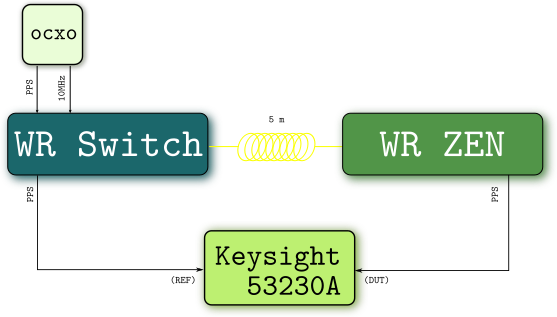
\includegraphics[width=\textwidth]{img/prueba1_pps.png}
        \caption{Setup for the PPS results of the WR-ZEN directly connected to the Grand Master WRS.}
        \label{fig:prueba1_sch}
    \end{subfigure}
    ~
    \begin{subfigure}[t]{.60\textwidth}
        \centering
        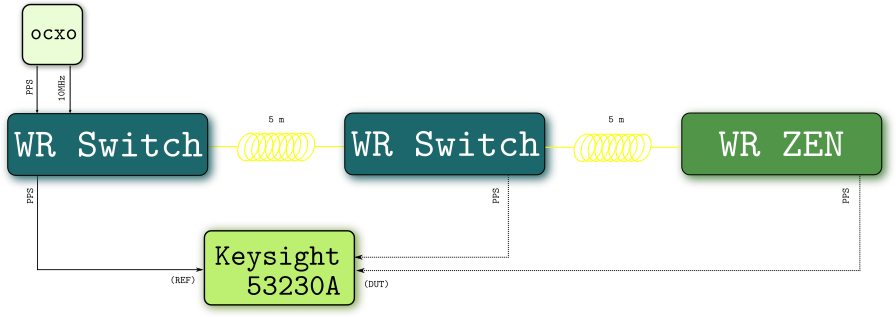
\includegraphics[width=\textwidth]{img/prueba2-3_pps.png}
        \caption{Setup for the network experiment taking measures from WRS L2 and the end node WR-ZEN.}
        \label{fig:prueba2_sch}
    \end{subfigure}
\end{figure}

Some long-term stability results are presented in table ?? and fig. \ref{fig:tdev_plots} because of the importance of that kind of measures for time distribution networks. This time, we have take the PPS outputs from WRS and WR-ZEN and we have performed some long time measurements and plotted them with a Time Deviation (TDEV) analysis.

\begin{figure}
    \begin{subfigure}[t]{.45\textwidth}
        \centering
        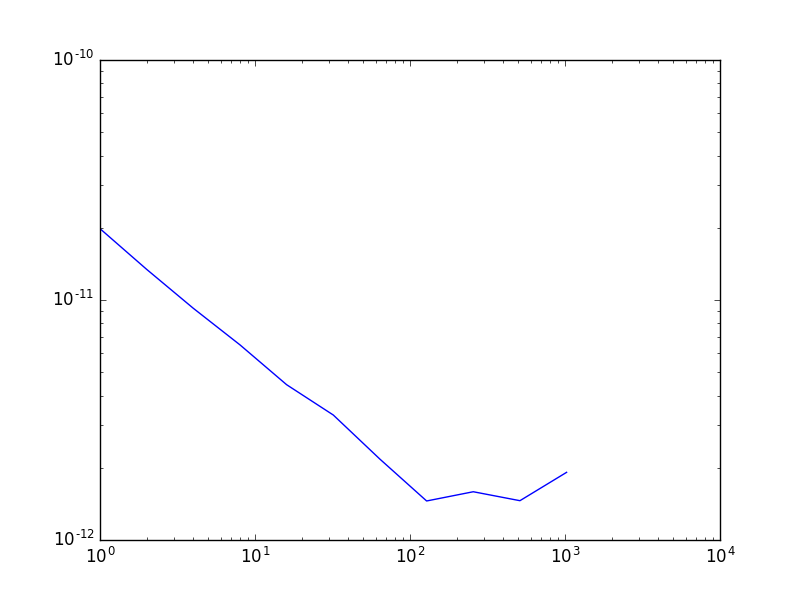
\includegraphics[width=\textwidth]{img/pps_p1.png}
        \caption{TDEV for the first configuration.}
        \label{fig:pps_p1}
    \end{subfigure}
    ~
    \begin{subfigure}[t]{.45\textwidth}
        \centering
        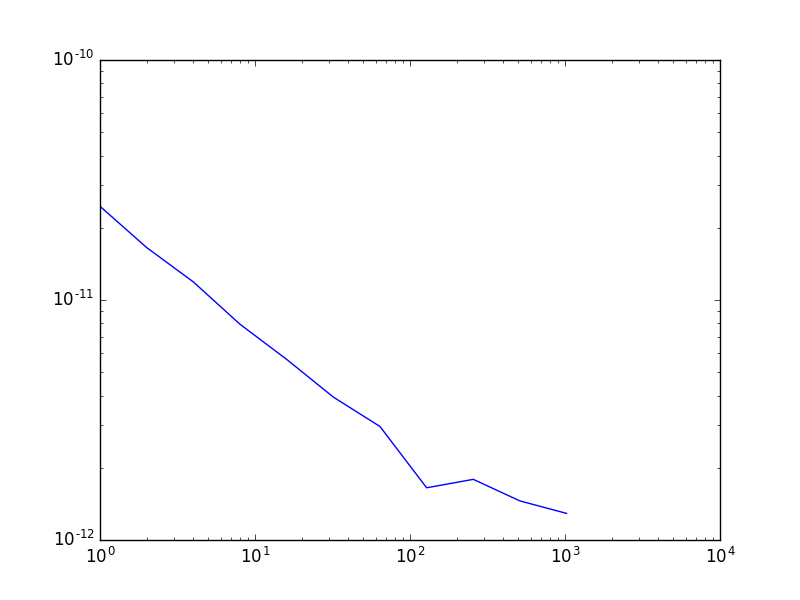
\includegraphics[width=\textwidth]{img/pps_p2.png}
        \caption{TDEV for the second configuration.}
        \label{fig:pps_p2}
    \end{subfigure}
    
    \centering
    \begin{subfigure}[t]{.45\textwidth}
        \centering
        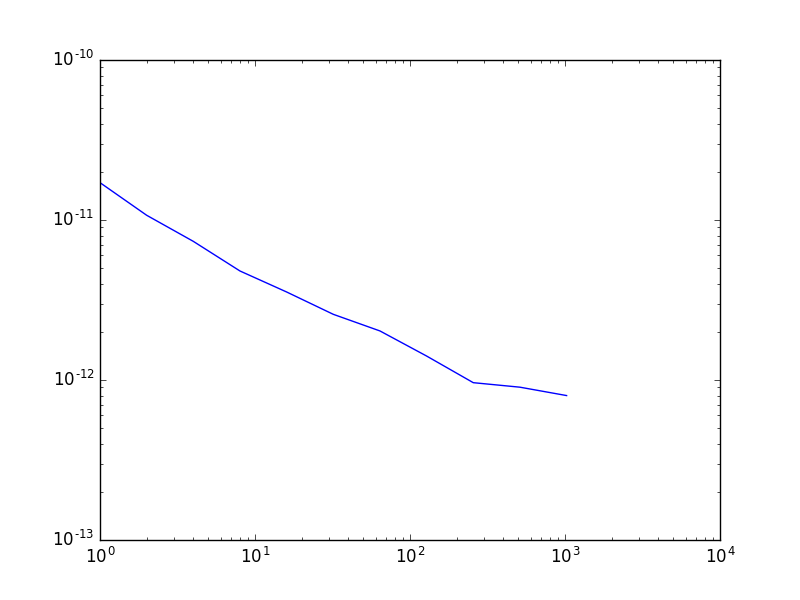
\includegraphics[width=\textwidth]{img/pps_p3.png}
        \caption{TDEV for the third configuration.}
        \label{fig:pps_p3}
    \end{subfigure}
    \caption{Time Deviation plots for the PPS distribution system}
    \label{fig:tdev_plots}
\end{figure}

\missingfigure{tabla MTIE}

\subsection{Traffic influence on synchronization accuracy}

% Posible experimento metiendo tráfico a la cadena anterior

\subsection{Redundancy}

% Este no me queda muy claro, cuando toque se verá

\subsection{Thermal characterization...}

% Aquí irían el de la cámara térmica, mover las fibras para simular viento y
% chorradas por el estilo

 


\section{Conclusion} \label{sec:conclusion}

In this contribution, we have presented an implementation of a high accuracy 
PPS distribution system based on the WR technology. The chosen platform for 
this device is the WR-ZEN which improves the previous existing WR node designs 
thanks to the inclusion of the FPGA-SoC platform and evolved hardware clocking 
circuitry. Thanks to the new architecture, the develop process is easier than 
in embedded platforms because a Linux kernel is used and allows you to abstract 
specific hardware details. Moreover, the flexibility of the system has been 
improved so that many clocking schemas can be test looking for the best 
synchronization quality results targeting the SKA needs.

One of the challenges of the SKA facilities is keeping the high accuracy 
synchronization through huge amount of nodes which are connected using long 
distance fibre links along dessert areas which present severe climatic 
conditions. In addition to that, SKA demands a strict timing requirements: a 
jitter in the tens of the picoseconds level and a time budget below 10 ns. 
However, not all of this budget is available for the PPS distribution system 
which needs to maintain the timing accuracy below 2ns. The proposed developed 
system creates a ecosystem with several applications, drivers and scripts that 
eases the user interaction with the rest of the 
SKA components providing synchronization but also allowing to extend the system 
capabilities through additional FMC cards.

We have also consider to evaluate the current PPS distribution system proposal 
in order to validate the developed solution for its inclusion in the SKA 
infrastructure. The results, given by the device performance evaluation tests, 
prove that the synchronization accuracy is bounded below 200ps which is far 
away from the 2ns SKA requirements. In addition to a device characterization, 
the evaluation of the scalability was an important result due to the high 
number of nodes in SKA1. We stated that a 2 level WR network is enough to 
synchronize all the expected nodes of the SKA system maintaining the required 
synchronization accuracy inside the SKA timing limits. Furthermore, we have 
designed several experiments simulating the SKA climatic place conditions 
looking for evaluating the thermal change influence in the propagation delay 
and its repercussion in the PPS distribution system. We observed that for a 
20ºC temperature difference the propagation delay is increased tens of 
nanoseconds (~ 96 ns) but the PPS offset keeps its accuracy with an offset that 
does not exceed the hundred of picoseconds (~ 211 ps). 

Finally, we can conclude with the presented results that the proposed PPS 
distribution system based on WR fulfil the expected timing requirement for SKA 
radio-telescope infrastructure.

\section{Future work} \label{sec:future-work}

The develop PPS distribution system is working at the moment but it is 
necessary to test in depth in the SKA places in order to check all the 
possible scenarios. Most important issues needing to be evaluated as part of 
the future work are: (i) the problem with the variable wavelength for the 
current chosen SPFs and their calibration; and (ii) the evaluation of the 
conditions where the WR equipment will be placed in order to detect if the 
temperature change can degrade significantly the PPS accuracy.

Moreover, the solution is flexible enough to be used in another first level 
scientific projects, so that, more specific tests should be performed in order 
to evaluate the developed platform for its inclusion in other projects.

\section{Acknowledgements} \label{sec:acknowledgments}

The authors would like to thank to the CERN BE-CO-HT group, the WR community, the Seven Solutions staff and
other institutions such as JIVE (especially Paul Boven) for its collaboration testing the
WR-ZEN board. This work has been partially funded by the Horizon 2020 (H2020) ASTERICS (grant number 653477),
VITVIR (TIC-8120, Junta de Andalucia) and AYA2015-65973-C3-2-R: "AMIGA6: gas in and around galaxies. Preparation for SKA science and contribution to the design of the SKA data flow. Signal and Data Transport (SaDT)" projects.

\section*{References}\label{sec:references}

\bibliography{mybibfile}

\end{document}
